\documentclass[11pt, handout]{beamer}

\usepackage[utf8]{inputenc}
\usepackage[francais]{babel}
\usepackage{tcolorbox}
\usepackage{minted}
\usepackage{pdfpages}
\usepackage{sourcecodepro}
\usepackage{graphicx}

% Scala
\newminted{scala}{frame=single, framesep=6pt, breaklines=true,
  fontsize=\scriptsize,gobble=2}
\newmintedfile{scala}{frame=single, framesep=6pt, breaklines=true,
  fontsize=\scriptsize}

% VHDL
\newminted{vhdl}{frame=single,framesep=6pt, breaklines=true,
  fontsize=\scriptsize}
\newmintedfile{vhdl}{frame=single, framesep=6pt, breaklines=true,
  fontsize=\scriptsize,gobble=2}

\usetheme{CambridgeUS}
\setbeamertemplate{\insertframenumber/\inserttotalframenumber}

\title[KlugHDL]{KlugHDL : a SpinalHDL diagram generator}
\subtitle[PA]{Défense de projet d'approfondissement}
\author{Sylvain Julmy}
\institute[MSE]{Institut Systèmes Industriels\\Master of Science HES-SO}
\date{\today}

\AtBeginSection[]{
  \begin{frame}
    \frametitle{Schedule}
    \tableofcontents[
    currentsubsection,
    sectionstyle=show/shaded,
    ]
  \end{frame}
}

\begin{document}

\maketitle

\begin{frame}
  \frametitle{Overview of contents}
    \tableofcontents[]
\end{frame}

\section{Context}

\begin{frame}
  \frametitle{VHDL}
  \begin{itemize}
  \item Hardware description language
  \item Mostly with Verilog for programming on the FPGA
  \item Old, verbose and tricky
  \end{itemize}
\end{frame}

\begin{frame}
  \frametitle{SpinalHDL}

  \begin{tcolorbox}
  SpinalHDL, written as an internal DSL, is used to describe digital hardware and generate the corresponding
  source code in VHDL (or Verilog).
  \end{tcolorbox}

\end{frame}

\begin{frame}[fragile]
  \frametitle{VHDL vs SpinalHDL}

  \begin{minipage}{0.45\textwidth}
  \begin{scalacode}
  import spinal.core._
  
  class AND extends Component {
    val io = new Bundle {
      val a = in Bool
      val b = in Bool
      val c = out Bool
    }
    io.c := io.a & io.b
  }
  \end{scalacode}
  \end{minipage}
  \hfill
  \begin{minipage}{0.45\textwidth}
  \begin{vhdlcode}
  entity AND_1 is
    port(
      io_a : in std_logic;
      io_b : in std_logic;
      io_c : out std_logic
    );
  end AND_1;
   
  architecture arch of AND_1 is
  begin
    io_c <= (io_a and io_b);
  end arch;
  \end{vhdlcode}
  \end{minipage}
\end{frame}

\begin{frame}
  \frametitle{KlugHDL}
  \begin{tcolorbox}
  An application which is able to analyse a SpinalHDL program and produce a
  block diagram of the corresponding hardware description.
  \end{tcolorbox}
\end{frame}

\begin{frame}
  \frametitle{KlugHDL}
  \begin{center}
  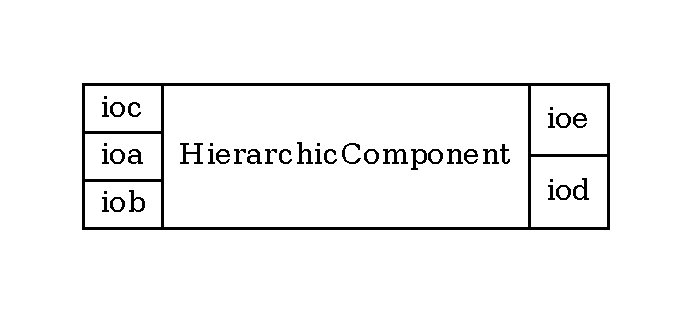
\includegraphics[width=0.8\textwidth]{hierarchic_component}
  \end{center}
\end{frame}

\begin{frame}
  \frametitle{KlugHDL}
  \begin{minipage}{0.30\textwidth}
  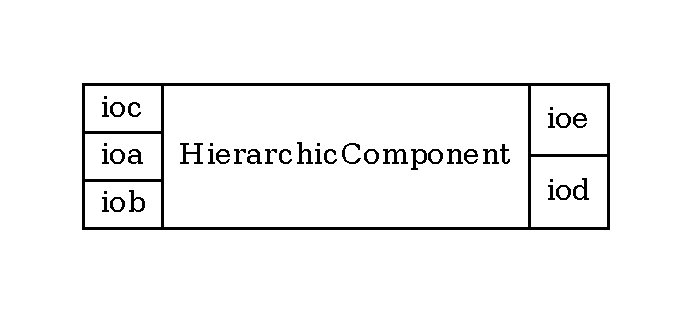
\includegraphics[width=1.0\textwidth]{hierarchic_component}
  \end{minipage}
  \hfill
  \begin{minipage}{0.69\textwidth}
  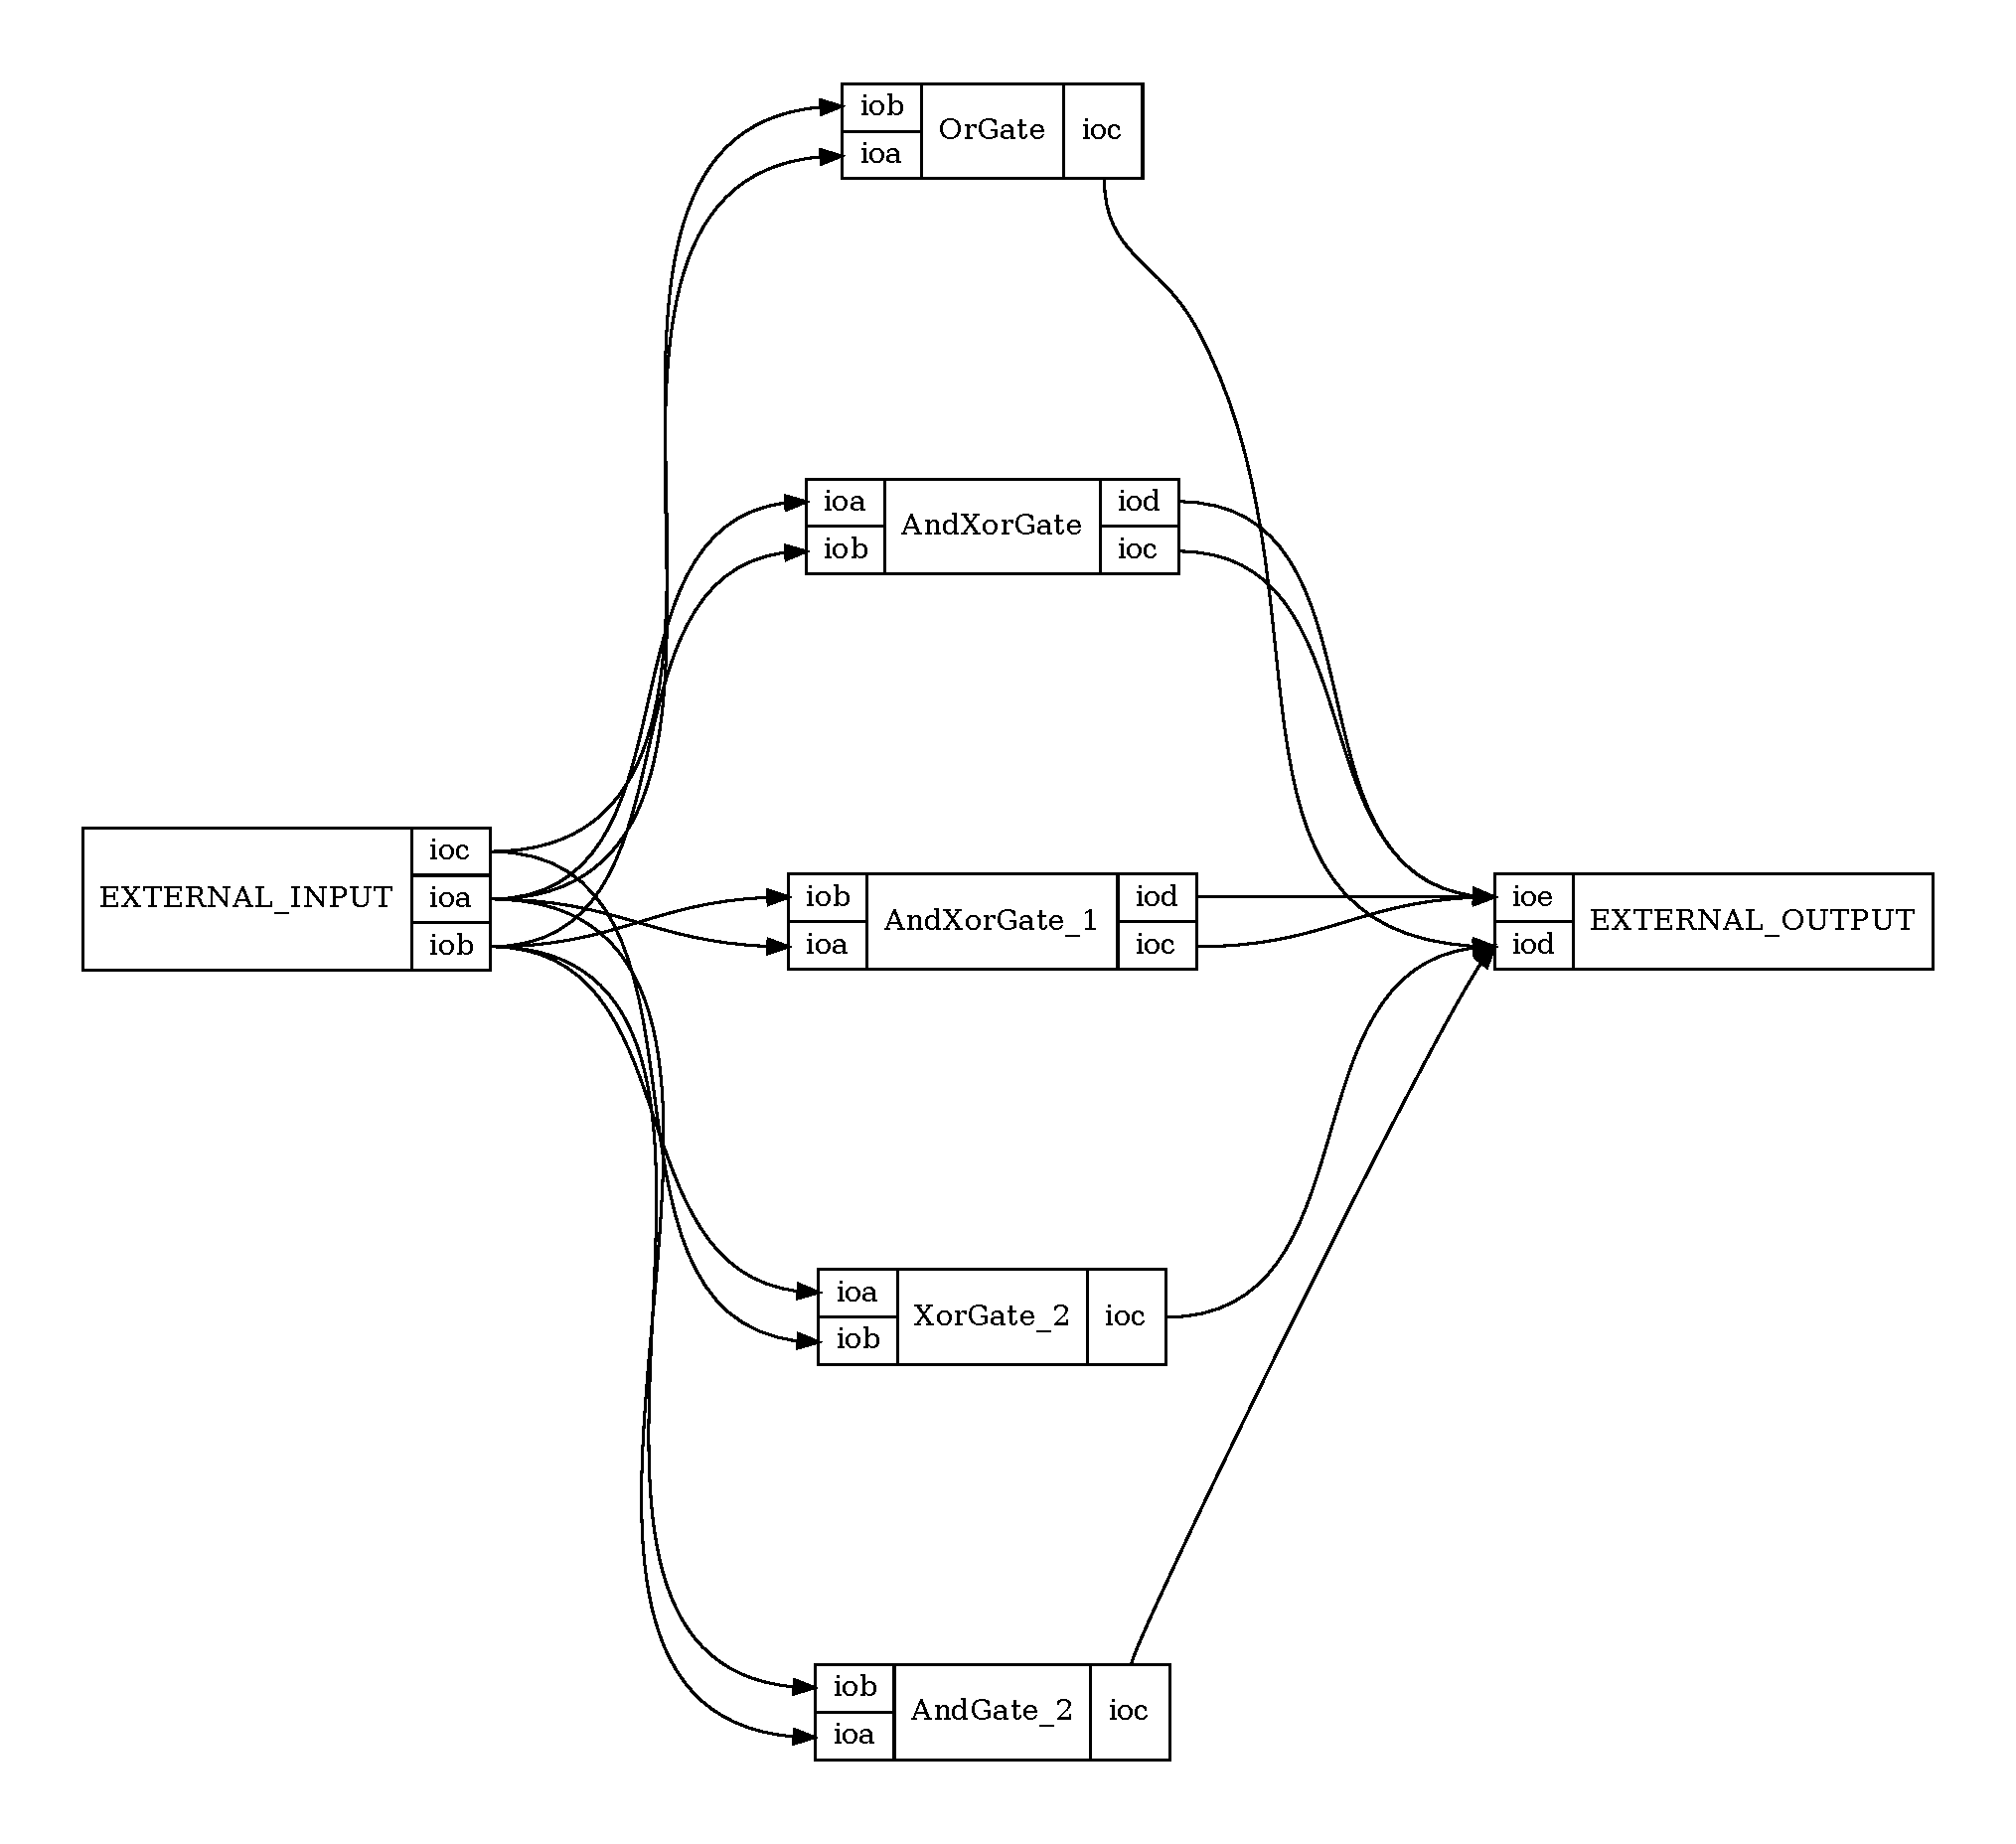
\includegraphics[width=1.0\textwidth]{hierarchic_component_inside}
  \end{minipage}
\end{frame}

\section{Diagrams modeling}

\section{Parsing the AST}

\section{Viewving library}

\section{Diagram visualization}

\section{Current working state}

\section{Further work}

\section{Conclusion}

\section{Questions}

\end{document}

%%% Local Variables:
%%% TeX-command-extra-options: "-shell-escape"
%%% TeX-master: t
%%% End:
